\chapter{Progettazione Concettuale}

\section{Progettazione Concettuale con Class Diagrams}

La progettazione concettuale è la fase in cui si modella il \textit{cosa} deve essere rappresentato nella base di dati, ignorando i dettagli implementativi del DBMS. Sebbene la letteratura classica utilizzi il modello Entity-Relationship (ER), l'approccio moderno predilige l'uso dei \textbf{Class Diagrams UML}, di cui di seguito richiameremo i concetti fondamentali. Si assumerà che il lettore abbia già familiarità con i diagrammi UML in un contesto orientato agli oggetti, dunque ne faremo dei richiami piuttosto sommari e ci concentreremo sulle specificità della modellazione per basi di dati.
\vspace{\baselineskip}

Il punto di partenza è un testo in linguaggio naturale (specifiche). La costruzione del diagramma segue una strategia di mapping semantico:

\begin{itemize}
    \item \textbf{Sostantivi $\rightarrow$ Classi (Entità):} Rappresentano oggetti con esistenza autonoma (es. \textit{Studente, Corso}).
    \item \textbf{Verbi $\rightarrow$ Associazioni (Relazioni):} Descrivono i legami logici tra le classi (es. \textit{Iscrive, Sostiene}).
    \item \textbf{Aggettivi o Specifiche $\rightarrow$ Attributi:} Proprietà atomiche che descrivono una classe (es. \textit{Nome, Matricola}).
\end{itemize}
\vspace{\baselineskip}

Gli elementi costitutivi di un Class Diagram sono:
\begin{description}
    \item[Classe:] Rappresentata da un rettangolo. Nella progettazione concettuale ci si concentra su \textit{Nome} e \textit{Attributi}. Le \textit{Operazioni} (metodi) vengono solitamente omesse.
    \item[Associazione:] Una linea che connette due classi. Indica che esiste una correlazione logica tra le istanze delle classi coinvolte.
    \item[Cardinalità:] Indicano il numero minimo e massimo di istanze di una classe che possono essere legate a una singola istanza della classe opposta.
\end{description}

\begin{table}[h]
    \centering
    \caption{Sintassi delle Cardinalità UML}
    \begin{tabular}{@{}ll@{}}
        \toprule
        \textbf{Sintassi} & \textbf{Significato} \\
        \midrule
        \texttt{1} & Esattamente uno (Obbligatorio) \\
        \texttt{0..1} & Zero o uno \\
        \texttt{*} o \texttt{0..*} & Zero o molti \\
        \texttt{1..*} & Uno o molti (Almeno uno) \\
        \bottomrule
    \end{tabular}
\end{table}

Un attributo si dice \textbf{totale} se ha cardinalità minima strettamente maggiore di zero, \textbf{parziale} altrimenti: quindi il primo deve sempre avere un valore, mentre per uno parziale il valore è opzionale. 

Un attributo si dice \textbf{singolo} se ha cardinalità massima uguale a uno, \textbf{multiplo} altrimenti.
\vspace{\baselineskip}

Un attributo è \textbf{atomico} se il database non ne percepisce la struttura interna. Gli attributi atomici possono essere:

\begin{itemize}
    \item \textbf{Primitivi}: Rappresentano valori elementari non scomponibili.
    \begin{itemize}
        \item \textit{Numerici}: \texttt{int, float, decimal}.
        \item \textit{Alfanumerici}: \texttt{string, char}.
        \item \textit{Logici}: \texttt{boolean}.
    \end{itemize}
    \item \textbf{Predefiniti Strutturati}: Tipi di dato complessi forniti dal sistema e trattati come atomici dal DBMS.
    \begin{itemize}
        \item \textit{Temporali}: \texttt{date, time, timestamp}.
        \item \textit{Oggetti Binari}: \texttt{blob} (immagini, file), \texttt{clob} (testi estesi).
    \end{itemize}
\end{itemize}
\vspace{\baselineskip}

Un errore comune è modellare come attributo ciò che dovrebbe essere una classe. La regola empirica è:
\begin{enumerate}
    \item Se l'informazione è un valore semplice (es. \textit{Età}), è un \textbf{Attributo}.
    \item Se l'informazione ha proprietà proprie o deve essere legata ad altre entità (es. \textit{Indirizzo} inteso come via, civico e CAP), deve essere una \textbf{Classe} autonoma.
\end{enumerate}

\begin{warningbox}[]
    L'insieme degli attributi deve permettere di identificare univocamente ogni istanza della classe.
\end{warningbox}

\begin{observation}
    Sebbene in Java usi \texttt{-} (private) e \texttt{+} (public), nei diagrammi per database la visibilità è meno rilevante, ma mantenere il - per gli attributi aiuta a ricordare l'incapsulamento dei dati.
\end{observation}

\section{Ruoli nelle Associazioni}

Un \textbf{ruolo} identifica la funzione specifica che un'istanza di una classe svolge all'interno di un'associazione. Viene indicato alle estremità della linea di associazione.

\begin{itemize}
    \item \textbf{Utilità}: I ruoli sono essenziali per chiarire il significato del legame, specialmente quando l'associazione è \textit{riflessiva} (connette una classe a sé stessa) o quando esistono più associazioni tra le stesse classi.
    \item \textbf{Naming Convention}: Solitamente si utilizza un sostantivo che descrive la responsabilità (es. \textit{responsabile, supervisore, partecipante}).
    \item \textbf{Corrispondenza OOP}: Nella programmazione ad oggetti, il nome del ruolo coincide spesso con il nome dell'attributo (o del campo) che contiene il riferimento all'oggetto correlato.
\end{itemize}

\begin{example}[Associazione Riflessiva o Ricorsiva]
    Si consideri la classe \texttt{Persona} e l'associazione \textit{Genitorialità}. Senza ruoli, il legame sarebbe ambiguo. Assegnando i ruoli \textbf{genitore} e \textbf{figlio} alle due estremità, la semantica del modello diventa univoca.
\end{example}

\begin{observation}
    Spesso si tende a omettere il nome dell'associazione (il verbo al centro della linea) se i ruoli sono già sufficientemente esplicativi. In molti schemi professionali vengono mostrati solo i ruoli, perché sono più vicini alla struttura logica finale del database.
\end{observation}

\section{Navigabilità e Direzionalità}

Una differenza cruciale tra la modellazione OOP e quella per basi di dati riguarda la \textbf{navigabilità} delle associazioni.

\begin{itemize}
    \item \textbf{In Java (OOP)}: Le associazioni sono spesso \textit{unidirezionali} per favorire il disaccoppiamento tra le classi. La direzione indica quale oggetto mantiene il riferimento (puntatore) verso l'altro.
    \item \textbf{Nelle Basi di Dati}: Le associazioni sono intrinsecamente \textit{bidirezionali}. Una relazione tra due entità rappresenta un fatto logico che può essere interrogato partendo da entrambi i lati (es. tramite operatori di \textit{Join} in SQL).
\end{itemize}

\medskip

Dunque nel class diagram concettuale per database, si evitano solitamente le frecce di navigabilità. Una linea semplice indica che l'informazione è disponibile per l'interrogazione in modo simmetrico. La "direzionalità" fisica verrà stabilita solo nella fase di progettazione logica attraverso il posizionamento delle chiavi esterne.


\section{Tipi Enumerativi (Enumerazioni)}

Quando il dominio di un attributo è costituito da un insieme di valori costante, discreto e predefinito, si utilizza il costrutto della \textbf{Enumerazione}. Si tratta di un tipo di dato speciale che permette a un attributo di assumere solo uno dei valori elencati in una lista chiusa.

In UML, le enumerazioni sono rappresentate come classi con lo stereotipo \guillemotleft enumeration\guillemotright. Non hanno attributi propri, ma contengono un elenco di valori letterali che rappresentano le possibili istanze del tipo enumerativo.

\section{Classi di Associazione}

Nella modellazione concettuale, capita spesso che un'associazione tra due classi possieda delle proprietà proprie. Se un attributo non descrive intrinsecamente né la classe A né la classe B, ma esiste solo in funzione della loro relazione, ci troviamo di fronte alla necessità di una \textbf{Classe di Associazione}.

Si consideri, ad esempio, il caso classico di un sistema universitario: uno \textbf{Studente} sostiene un \textbf{Corso}. Vogliamo memorizzare il \textit{voto} conseguito.
\begin{itemize}
    \item Il \textit{voto} non è un attributo dello \texttt{Studente} (egli ha voti diversi per corsi diversi).
    \item Il \textit{voto} non è un attributo del \texttt{Corso} (il corso ha voti diversi per studenti diversi).
\end{itemize}

In un diagramma standard, saremmo costretti a omettere il voto o a inserirlo forzatamente in una delle due classi, creando un errore concettuale e ridondanza.

% Diagramma 1: Relazione molti-a-molti senza attributi
% [Codice PlantUML 1]
\begin{figure}[htbp] 
    \centering
    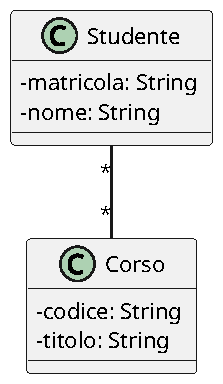
\includegraphics[width=0.2\textwidth]{immagini/cap01_im01.pdf} 
    \caption{Associazione Studente-Corso.}
\end{figure}

L'UML risolve il problema permettendo a un'associazione di avere una propria classe collegata. Questa classe ha un doppio valore: è sia un legame logico tra le istanze, sia un contenitore di attributi.

% Diagramma 2: Classe di associazione (Esame)
% [Codice PlantUML 2]
\begin{figure}[htbp] 
    \centering
    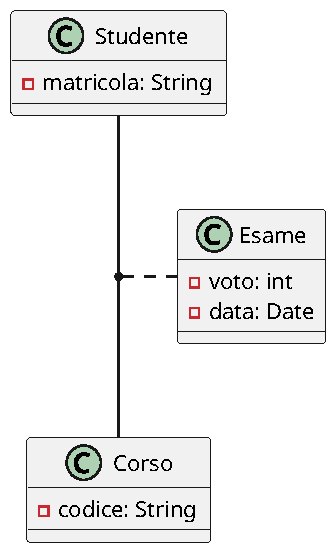
\includegraphics[width=0.3\textwidth]{immagini/cap01_im02.pdf} 
    \caption{Studente-Corso con classe di associazione Esame.}
\end{figure}

Sintatticamente, si rappresenta con un rettangolo di classe collegato alla linea di associazione tramite una \textbf{linea tratteggiata}. Essa eredita implicitamente le "chiavi" di entrambe le classi coinvolte.

In molte fasi di progettazione logica, o per chiarezza di implementazione, la classe di associazione viene "esplicitata" (o reificata). La classe di associazione diventa una classe intermedia a tutti gli effetti, e l'associazione molti-a-molti originale si trasforma in due associazioni uno-a-molti.

% Diagramma 3: Classe esplicitata
% [Codice PlantUML 3]
\begin{figure}[htbp] 
    \centering
    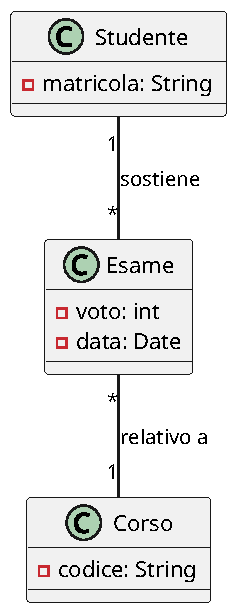
\includegraphics[width=0.2\textwidth]{immagini/cap01_im03.pdf} 
    \caption{Reificazione della classe di associazione Esame.}
    \label{fig:studente_corso}
\end{figure}

L'esplicitazione è spesso necessaria perché molti strumenti di modellazione o linguaggi di programmazione non supportano nativamente il costrutto della classe di associazione. In questo caso, la classe intermedia (es. \texttt{Esame}) funge da "ponte" tra le due entità principali.

\begin{tip}
    La classe di associazione è significativa solo su associazioni \textit{molti-a-molti}, ma occasionalmente si usa anche per altri tipi di associazioni. 
\end{tip}

\section{Grado di un'Associazione e Relazioni Ternarie}

Il \textbf{grado} di un'associazione è definito come il numero di classi coinvolte nel legame logico. 
\begin{itemize}
    \item \textbf{Associazioni Binarie (Grado 2):} Collegano due classi. Costituiscono la quasi totalità delle relazioni in un database.
    \item \textbf{Associazioni N-arie (Grado $N \ge 3$):} Collegano tre o più classi contemporaneamente. Il caso più comune è l'associazione \textbf{ternaria}.
\end{itemize}

\medskip

Un'associazione ternaria si rende necessaria quando il legame logico esiste solo se si considerano tre entità simultaneamente; la scomposizione in relazioni binarie separate causerebbe una perdita irreparabile di informazione semantica. In UML si rappresenta graficamente interponendo un \textbf{rombo} tra le linee che collegano le tre classi.

Si consideri, ad esempio, uno scenario di logistica industriale in cui sono coinvolte tre classi: \texttt{Fornitore}, \texttt{Prodotto} e \texttt{Progetto} (cantiere di destinazione). 
L'atto del rifornimento è un evento atomico: il \textit{Fornitore A} fornisce il \textit{Prodotto X} specificamente per il \textit{Progetto Y}. Se provassimo a mappare questo dominio con tre relazioni binarie (\textit{Fornitore-Prodotto}, \textit{Prodotto-Progetto}, \textit{Fornitore-Progetto}), sapremmo quali prodotti vende un fornitore e quali prodotti usa un progetto, ma non sapremmo mai \textbf{quale specifico fornitore ha portato quel determinato prodotto a quel singolo progetto}.

% Diagramma 4: Esempio associazione ternaria
% [Codice PlantUML 4]
\begin{figure}[htbp] 
    \centering
    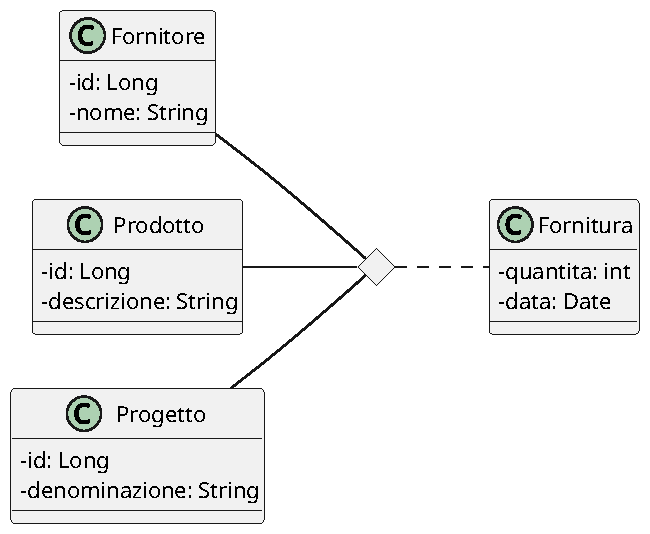
\includegraphics[width=0.5\textwidth]{immagini/cap01_im04.pdf} 
    \caption{Esempio associazione ternaria con classe di associazione.}
    \label{fig:ass_tern}
\end{figure}

\begin{tip}[Interpretazione di una associazione n-aria]
Per comprendere a fondo l'associazione ternaria, si può pensare che una delle tre classi non si colleghi singolarmente alle altre due, ma alla loro \textbf{coppia}. Nel nostro esempio, il \texttt{Progetto} non è legato separatamente a un \texttt{Prodotto} e a un \texttt{Fornitore}, ma è associato stabilmente alla coppia $(Prodotto, Fornitore)$, intesa come specifica combinazione. Analogamente per le altre due classi. 
\end{tip}

Poiché i DBMS relazionali e i framework ORM (come JPA/Hibernate) non supportano le relazioni native a tre vie, si deve \textbf{esplicitare} (o reificare) l'associazione prima dell'implementazione.

La reificazione trasforma il rombo dell'associazione in una classe vera e propria, che chiameremo \texttt{AssegnazioneFornitura}. L'associazione ternaria originale viene così frantumata in tre associazioni binarie distinte di tipo \textbf{1-a-Molti}:
\begin{itemize}
    \item Da \texttt{Fornitore} a \texttt{AssegnazioneFornitura} (Cardinalità \texttt{1} $\rightarrow$ \texttt{*})
    \item Da \texttt{Prodotto} a \texttt{AssegnazioneFornitura} (Cardinalità \texttt{1} $\rightarrow$ \texttt{*})
    \item Da \texttt{Progetto} a \texttt{AssegnazioneFornitura} (Cardinalità \texttt{1} $\rightarrow$ \texttt{*})
\end{itemize}

% Diagramma 5: Reificazione associazione ternaria
% [Codice PlantUML 5]
\begin{figure}[htbp] 
    \centering
    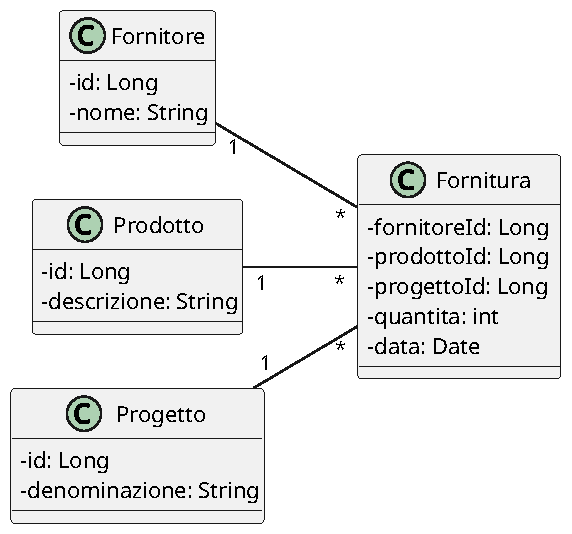
\includegraphics[width=0.5\textwidth]{immagini/cap01_im05.pdf} 
    \caption{Reificazione dell'associazione ternaria.}
    \label{fig:reif_ass_tern}
\end{figure}

Nella realtà, gli eventi n-ari catturano quasi sempre proprietà quantitative. Riprendendo l'esempio precedente, l'atto della fornitura genera intrinsecamente una \textit{quantità} di pezzi consegnati e una \textit{data} di consegna. Questi attributi non appartengono a nessuna delle tre classi isolate, ma alla loro combinazione. In UML si modella una \textbf{Classe di Associazione} (es. \texttt{Fornitura}) collegata tramite una linea tratteggiata al rombo dell'associazione ternaria.

Il processo di esplicitazione in questo scenario è immediato: la classe di associazione \texttt{Fornitura} viene promossa a classe centrale del cluster, inglobando gli attributi \texttt{quantità} e \texttt{data}. Le tre classi originarie si collegano a essa tramite relazioni binarie dirette.

\begin{warningbox}[La trappola delle cardinalità ternarie]
Nelle associazioni ternarie UML, la cardinalità posta vicino a una classe (es. \texttt{Progetto}) indica quante istanze di quella classe possono combinarsi con una \textbf{coppia fissa} di istanze delle altre due classi (\texttt{Fornitore} e \texttt{Prodotto}). Questa logica è controintuitiva e differisce dai diagrammi ER classici (notazione di Chen), inducendo spesso i progettisti in errore. Sostituire subito la ternaria con una classe esplicitata azzera ogni ambiguità interpretativa.
\end{warningbox}

\section{Aggregazione e Composizione}

Nello sviluppo dei Class Diagrams, le associazioni standard indicano un legame logico simmetrico. Tuttavia, per modellare scenari in cui esiste un rapporto di possesso o di subordinazione strutturale, l'UML introduce le \textbf{relazioni tutto-parte} (part-whole relationships). Queste si dividono in due varianti fondamentali, distinte in base al vincolo sul ciclo di vita degli oggetti coinvolti: l'aggregazione e la composizione.

L'\textbf{aggregazione} rappresenta una relazione in cui un oggetto ``Tutto'' (aggregante) contiene o colleziona uno o più oggetti ``Parte'' (aggregati), ma questi ultimi mantengono un'esistenza autonoma all'interno del dominio. Si tratta di un legame \textit{``has-a''} ad accoppiamento debole.

\begin{itemize}
    \item \textbf{Sintassi UML:} Si rappresenta graficamente con una linea che termina con un \textbf{rombo vuoto} (bianco) posizionato sul lato della classe ``Tutto''.
    \item \textbf{Ciclo di vita:} La distruzione dell'oggetto aggregante \textbf{non} comporta la distruzione degli oggetti aggregati.
\end{itemize}

\begin{example}[Università e Professore]
Si consideri la classe \texttt{Universita} (il Tutto) e la classe \texttt{Professore} (la Parte). Un'università raccoglie un insieme di docenti. Tuttavia, se l'università dovesse cessare la sua attività, i singoli professori non verrebbero eliminati dal sistema: essi continuerebbero ad esistere come entità autonome e potrebbero essere associati ad altri atenei.
\end{example}

% Diagramma 6: aggregazione
% [Codice PlantUML 6]
\begin{figure}[htbp] 
    \centering
    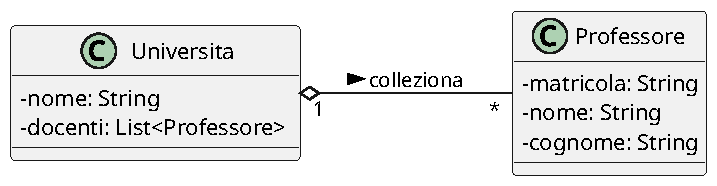
\includegraphics[width=0.5\textwidth]{immagini/cap01_im06.pdf} 
    \caption{Esempio di aggregazione}
\end{figure}



La \textbf{composizione} è una forma di aggregazione più stringente, esclusiva e gerarchica. In questo scenario, l'oggetto ``Parte'' è una componente indissolubile del ``Tutto''. Una parte può appartenere a un solo tutto alla volta e non ha alcuna autonomia esistenziale.

\begin{itemize}
    \item \textbf{Sintassi UML:} Si rappresenta con una linea che termina con un \textbf{rombo pieno} (nero) posizionato sul lato della classe ``Tutto''.
    \item \textbf{Ciclo di vita:} Il ciclo di vita delle parti è totalmente subordinato a quello del tutto. Di conseguenza, la distruzione dell'oggetto composto (Tutto) determina l'istanza di \textbf{distruzione automatica} di tutte le sue parti. La cardinalità dal lato del tutto è rigorosamente \texttt{1} o \texttt{0..1}.
\end{itemize}

\begin{example}[Ordine ed Elemento d'Ordine]
Si consideri un sistema di e-commerce con le classi \texttt{Ordine} (il Tutto) e \texttt{RigaOrdine} (la Parte, che descrive il prodotto e la quantità). Una riga d'ordine ha significato logico solo se contestualizzata all'interno dello specifico acquisto. Se l'utente decide di eliminare l'intero \texttt{Ordine}, il sistema deve rimuovere a cascata tutte le relative istanze di \texttt{RigaOrdine}.
\end{example}

% Diagramma 7: aggregazione
% [Codice PlantUML 7]
\begin{figure}[htbp] 
    \centering
    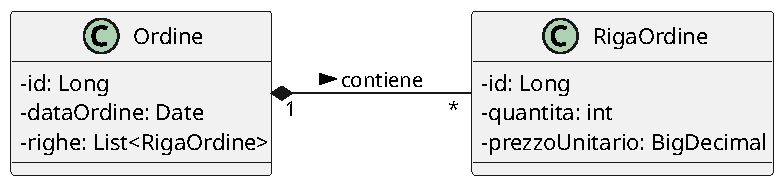
\includegraphics[width=0.5\textwidth]{immagini/cap01_im07.pdf} 
    \caption{Esempio di composizione}
\end{figure}

\begin{dettagli}[]
    L'aggregazione non ha alcuna necessità tecnica stringente: una semplice associazione fa esattamente lo stesso identico lavoro. A livello di tabelle, sia un'associazione generica sia un'aggregazione si tradurranno nello stesso modo, la differenza è puramente semantica e documentale, non implementativa. Alcuni autorevoli ingegneri del software (tra cui Martin Fowler, uno dei padri dell'architettura software moderna) sostengono da anni che l'aggregazione UML sia fondamentalmente inutile perché la linea di demarcazione con l'associazione standard è troppo sfumata e crea più ambiguità che benefici. Fowler la definisce ironicamente "un effetto placebo grafico".

    Il caso della composizione è invece più significativo, perché il diagramma fornisce un'informazione in più: la parte non può esistere senza il tutto. 
\end{dettagli}

\section{Generalizzazione ed Ereditarietà}

La \textbf{generalizzazione} (o ereditarietà) modella una relazione di tipo \textit{``IS-A''} (è-un) tra una classe più generale, detta \textbf{Superclasse} (o classe padre), e una o più classi più specifiche, dette \textbf{Subclassi} (o classi figlie). 

Le subclassi ereditano automaticamente tutti gli attributi, i ruoli e le associazioni della superclasse, senza necessità di ridefinirli, e possono estendere il modello introducendo attributi o associazioni propri.

\textbf{Sintassi UML:} Si rappresenta graficamente con una linea che termina con una \textbf{freccia con la punta triangolare vuota} rivolta verso la superclasse.

% Diagramma 8: aggregazione
% [Codice PlantUML 8]
\begin{figure}[htbp] 
    \centering
    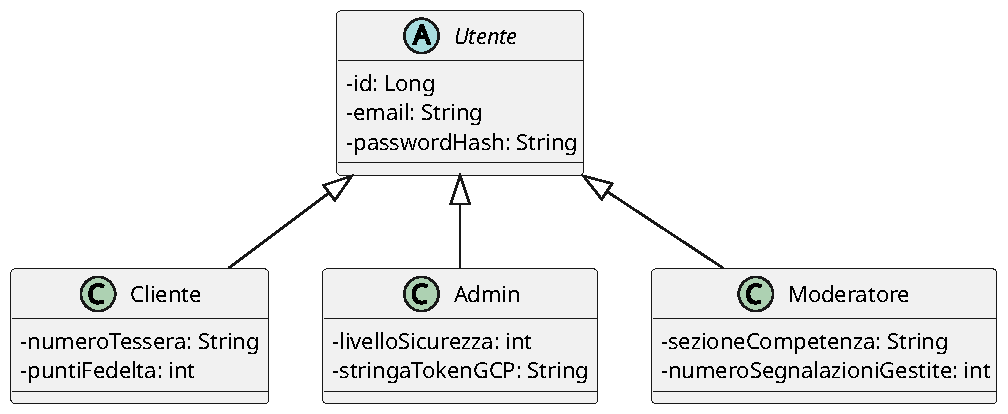
\includegraphics[width=0.7\textwidth]{immagini/cap01_im08.pdf} 
    \caption{Esempio di ereditarietà}
\end{figure}

È fondamentale comprendere che \textbf{l'ereditarietà non esiste nel modello relazionale delle basi di dati}. I database relazionali non possiedono strutture gerarchiche native; essi conoscono esclusivamente il concetto di tabella (relazione), che è per sua natura una struttura ``piatta'' e bidimensionale. 

La generalizzazione appartiene quindi in modo esclusivo al livello della \textbf{progettazione concettuale}. In questa fase, lo scopo del Class Diagram è modellare il dominio reale nel modo più fedele e naturale possibile, catturandone la semantica e i vincoli logici (ovvero i rapporti di sotto-tipo/sopra-tipo) ed eliminando qualsiasi vincolo tecnologico. Il problema di come ``appiattire'' questa gerarchia per adattarla a un database relazionale sarà l'obiettivo centrale della successiva fase di progettazione logica.




